\documentclass[handout,aspectratio=169]{beamer}
\usetheme{Montpellier}
\usecolortheme[snowy]{owl}

%%% Footline %%%
%\setbeamercolor{title in head/foot}{parent=footlinecolor}
\setbeamercolor{author in head/foot}{parent=footlinecolor1}
\setbeamercolor{date in head/foot}{parent=footlinecolor1}

%%%% headline %%%%
\setbeamercolor{title in head/foot}{fg=white, bg=black}
\setbeamercolor{section in head/foot}{fg=white, bg=black}
\setbeamercolor{subsection in head/foot}{fg=white, bg=black}
%\setbeamercolor{separation line}{bg=black}
%\setbeamercolor{section in head/foot}{fg=white, bg=black}
%\useoutertheme[subsection=false]{miniframes}

\usepackage{graphicx}
\usepackage{media9}
\usepackage{multimedia}
 \usepackage{siunitx}
\DeclareGraphicsExtensions{.jpg,.mps,.pdf,.png,.tif} % Formats d'Images
\setbeamercovered{dynamic}

\usepackage{environ}

\newcommand{\halfmargin}{0.05\paperwidth}
\newcommand{\margin}{0.10\paperwidth}

\beamersetrightmargin{\margin}
\beamersetleftmargin{\margin}

\NewEnviron{wideframe}[1][]{%
\begin{frame}{#1}
\makebox[\textwidth][c]{
\begin{minipage}{\dimexpr\paperwidth-\halfmargin-\halfmargin\relax}
\BODY
\end{minipage}}
\end{frame}
}

%\setcounter{secnumdepth}{0} \linespread{1.5}

\title[Spike Train Analysis]{Spike Train Analysis}
\author[Pierre Le Merre]{Pierre Le Merre}
\institute[]{CNRS, Centre de Recherche en Neuroscience de Lyon\\
Dept. of Neuroscience, Karolinska Institute}
\date[20261125]{GDR Minischool 2026\\
Paris - 25th of November 2026}


\begin{document}

% Gestion de la reprise du plan en cours de route

  \AtBeginSection[] % Do nothing for \subsection*
  {
   \begin{frame}
      \frametitle{Plan}
      \setcounter{tocdepth}{1}
      \tableofcontents[currentsection]
      \setcounter{tocdepth}{2}
    \end{frame}
 }
  \AtBeginSubsection[] % Do nothing for \subsection*
  {
    \begin{frame}
      \frametitle{Detailed plan}
      \tableofcontents[sectionstyle=show/hide,subsectionstyle=show/shaded/hide]
    \end{frame}
  }



% Slide de Titre
 \begin{frame}[plain]
   \titlepage
 \end{frame}
 
 
 %%%%%%%%%%%%%%%%%%%%%%%%%%%%%%%%%%%%%%%%%%%%%%%%%%%%%%%%%%%%%%%%%%%%%%%%%%%%%

\section[Introduction]{Introduction}

\begin{frame}
	\frametitle{Position of the problem}
		\begin{columns}
		\column{8cm}
		\begin{center}
			\begin{itemize}
  				\item Preprocessing is done (spike sorting, histology, behavior,...)
  				\item We have unit spike trains and other timestamps stored in some format...
  				\item %We have a research question. 
			\end{itemize}
		\end{center}
		\column{6cm}
		\begin{center}
				%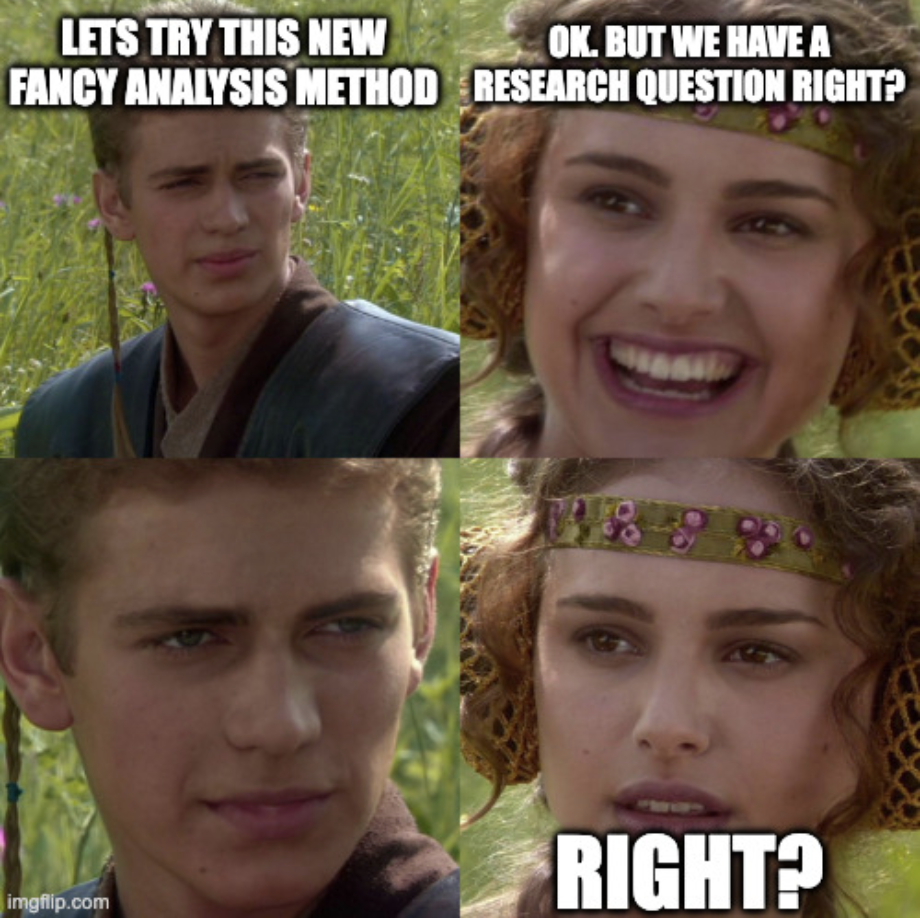
\includegraphics[width=6cm]{figures/padme.png}
		\end{center}
	\end{columns}
\end{frame} 

\begin{frame}
	\frametitle{Position of the problem}
		\begin{columns}
		\column{8cm}
		\begin{center}
			\begin{itemize}
  				\item Preprocessing is done (spike sorting, histology, behavior,...)
  				\item We have unit spike trains and other timestamps stored in some format...
  				\item We have a research question. 
			\end{itemize}
		\end{center}
		\column{6cm}
		\begin{center}
				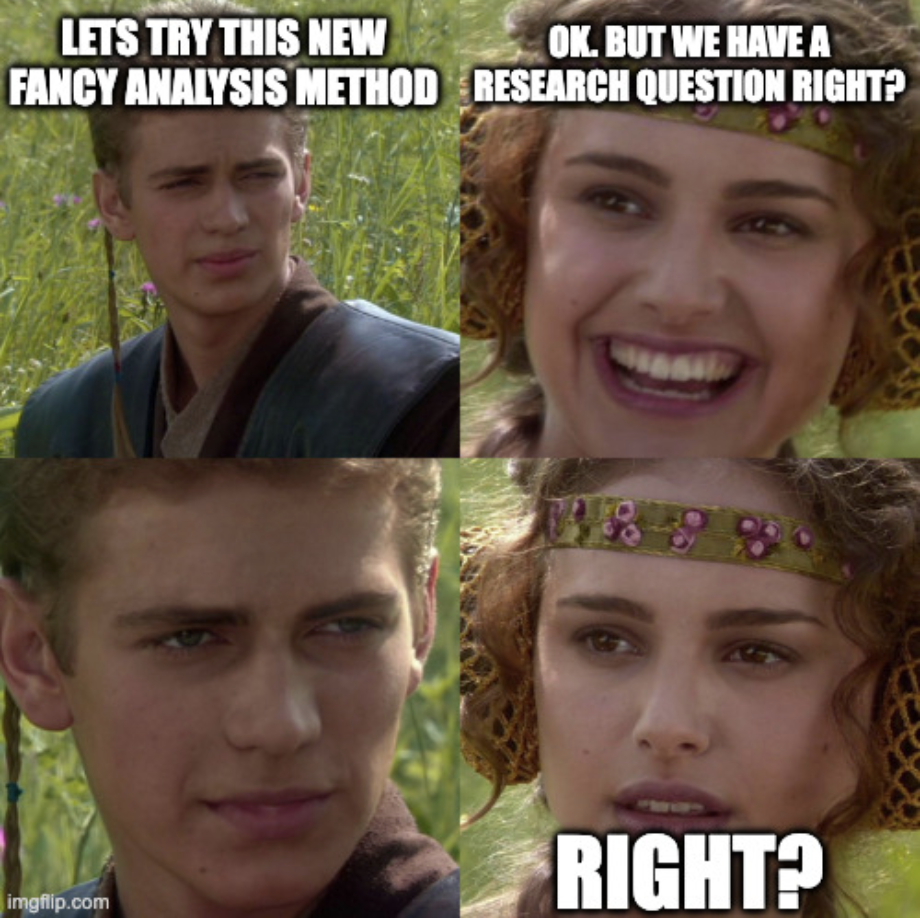
\includegraphics[width=6cm]{figures/padme.png}
		\end{center}
	\end{columns}
\end{frame} 


 %%%%%%%%%%%%%%%%%%%%%%%%%%%%%%%%%%%%%%%%%%%%%%%%%%%%%%%%%%%%%%%%%%%%%%%%%%%%%

\section[Setup]{Installation instructions}


\begin{frame}
\frametitle{Installation instructions}
Go to $\Rightarrow$ \url{https://github.com/PierreLeMerre/Minischool_GDR2026_SpikeTrains}
			\begin{center}
				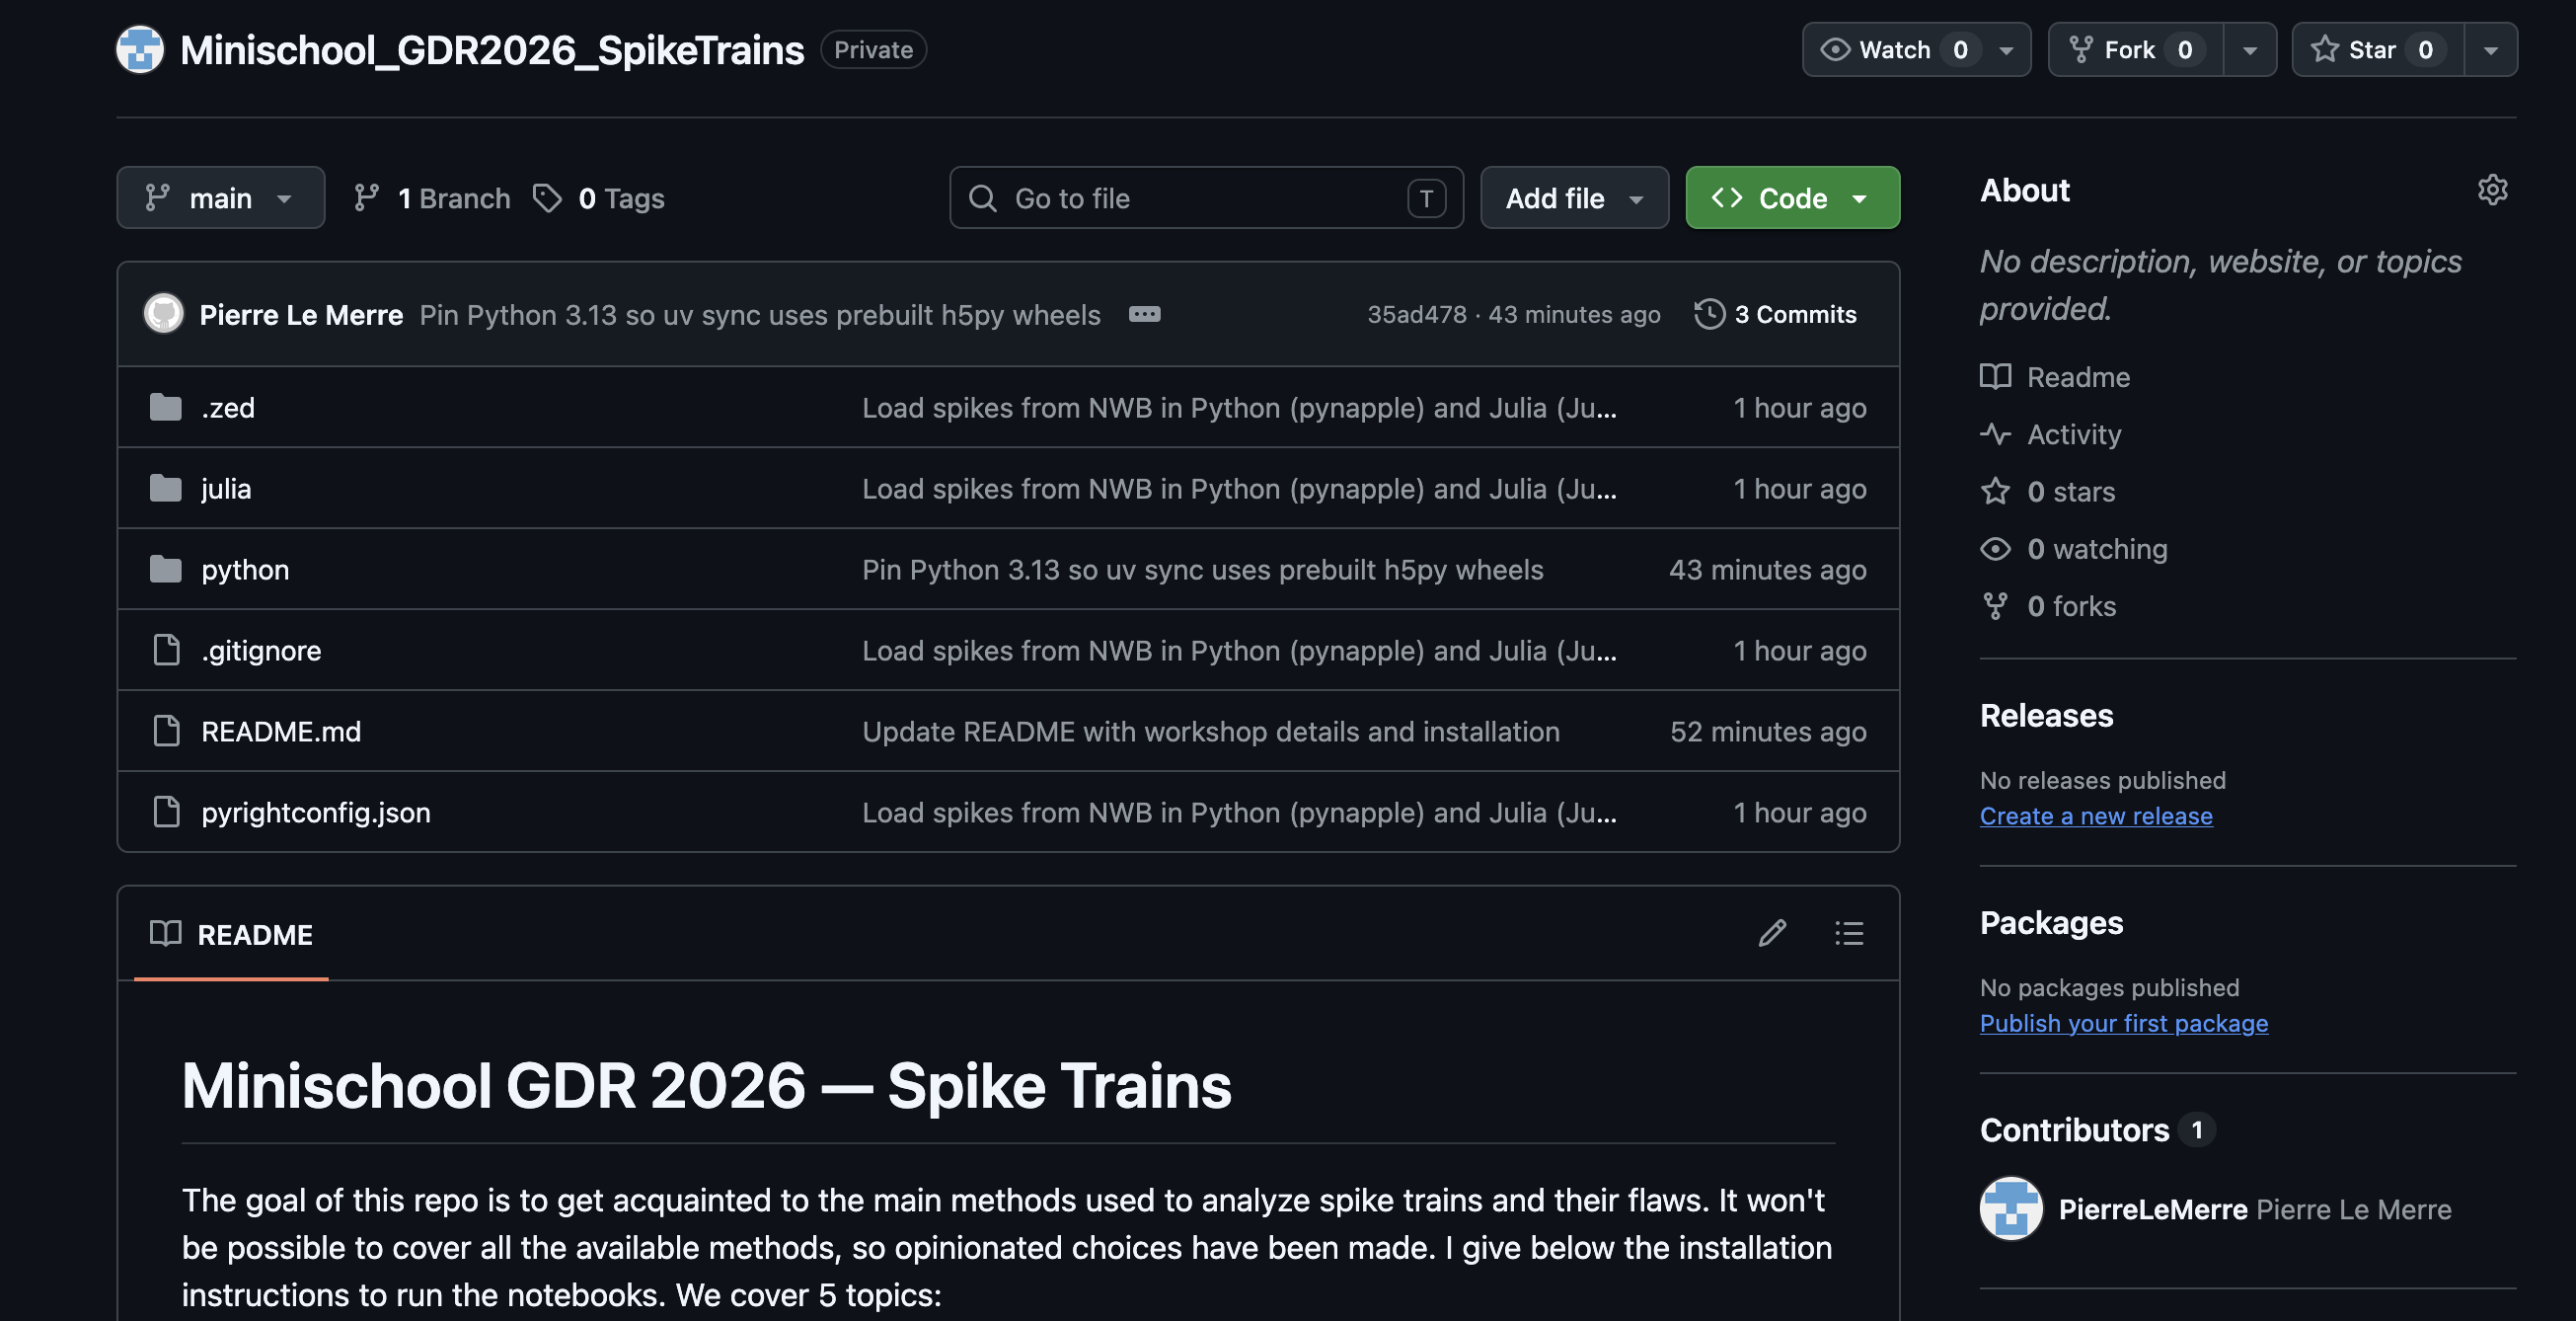
\includegraphics[width=8cm]{figures/repo.png}
			\end{center}
\end{frame} 


\begin{frame}
\frametitle{Download the data - Proposed framework}
			\begin{center}
				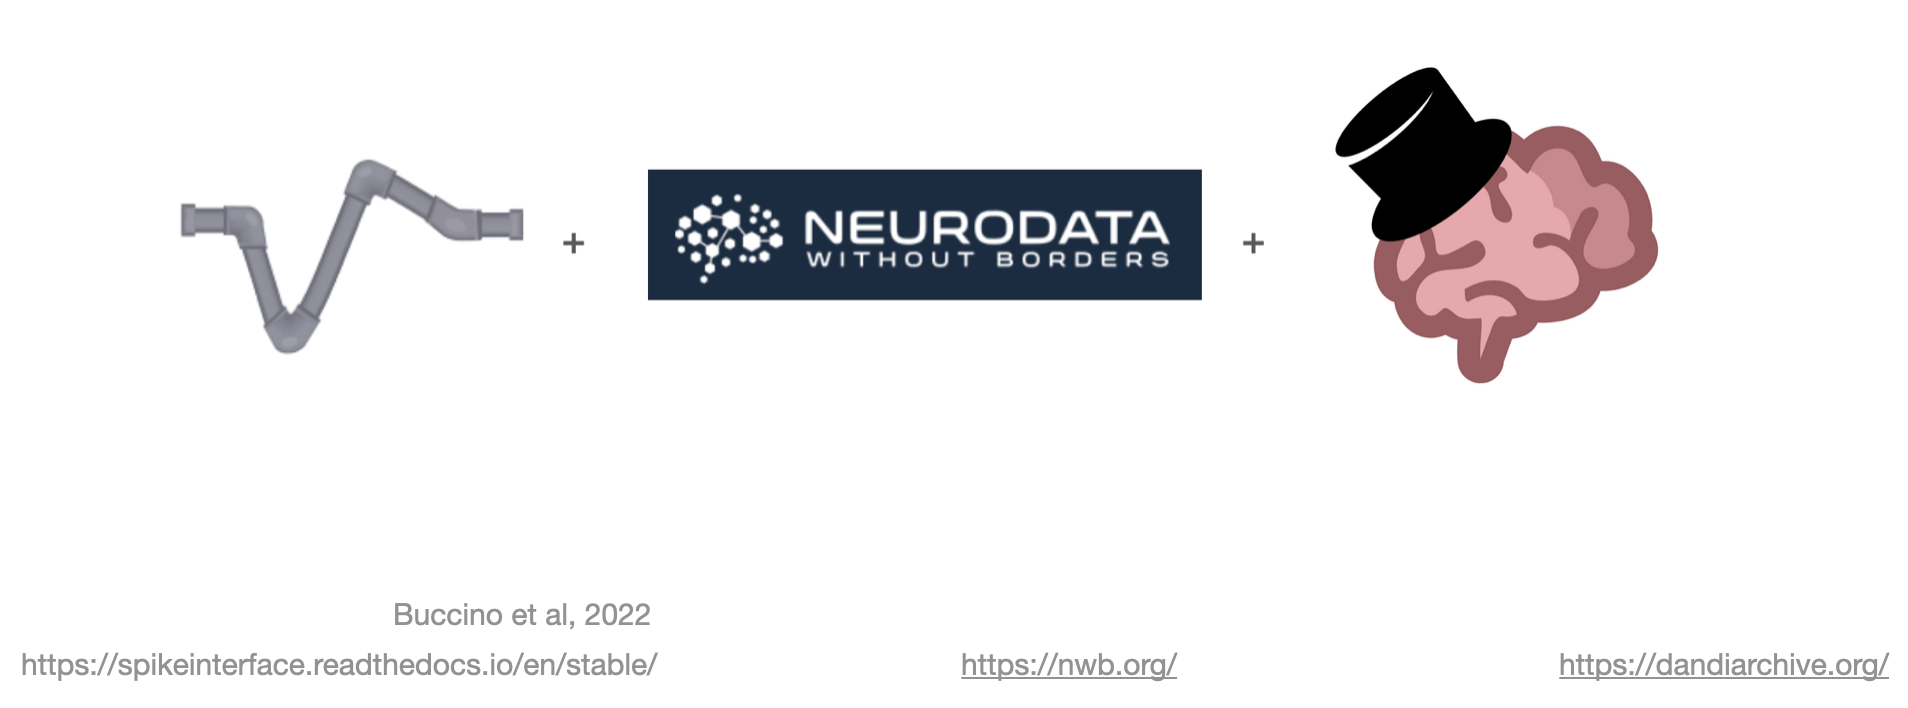
\includegraphics[width=14cm]{figures/eco.png}
			\end{center}
\end{frame} 

\begin{frame}
\frametitle{Download the data}
			\begin{center}
				link 2 data
			\end{center}
\end{frame} 

\begin{frame}
\frametitle{Explore NWB data - HDFView}
\url{https://github.com/HDFGroup/hdfview/releases/tag/v3.5.0}
			\begin{center}
				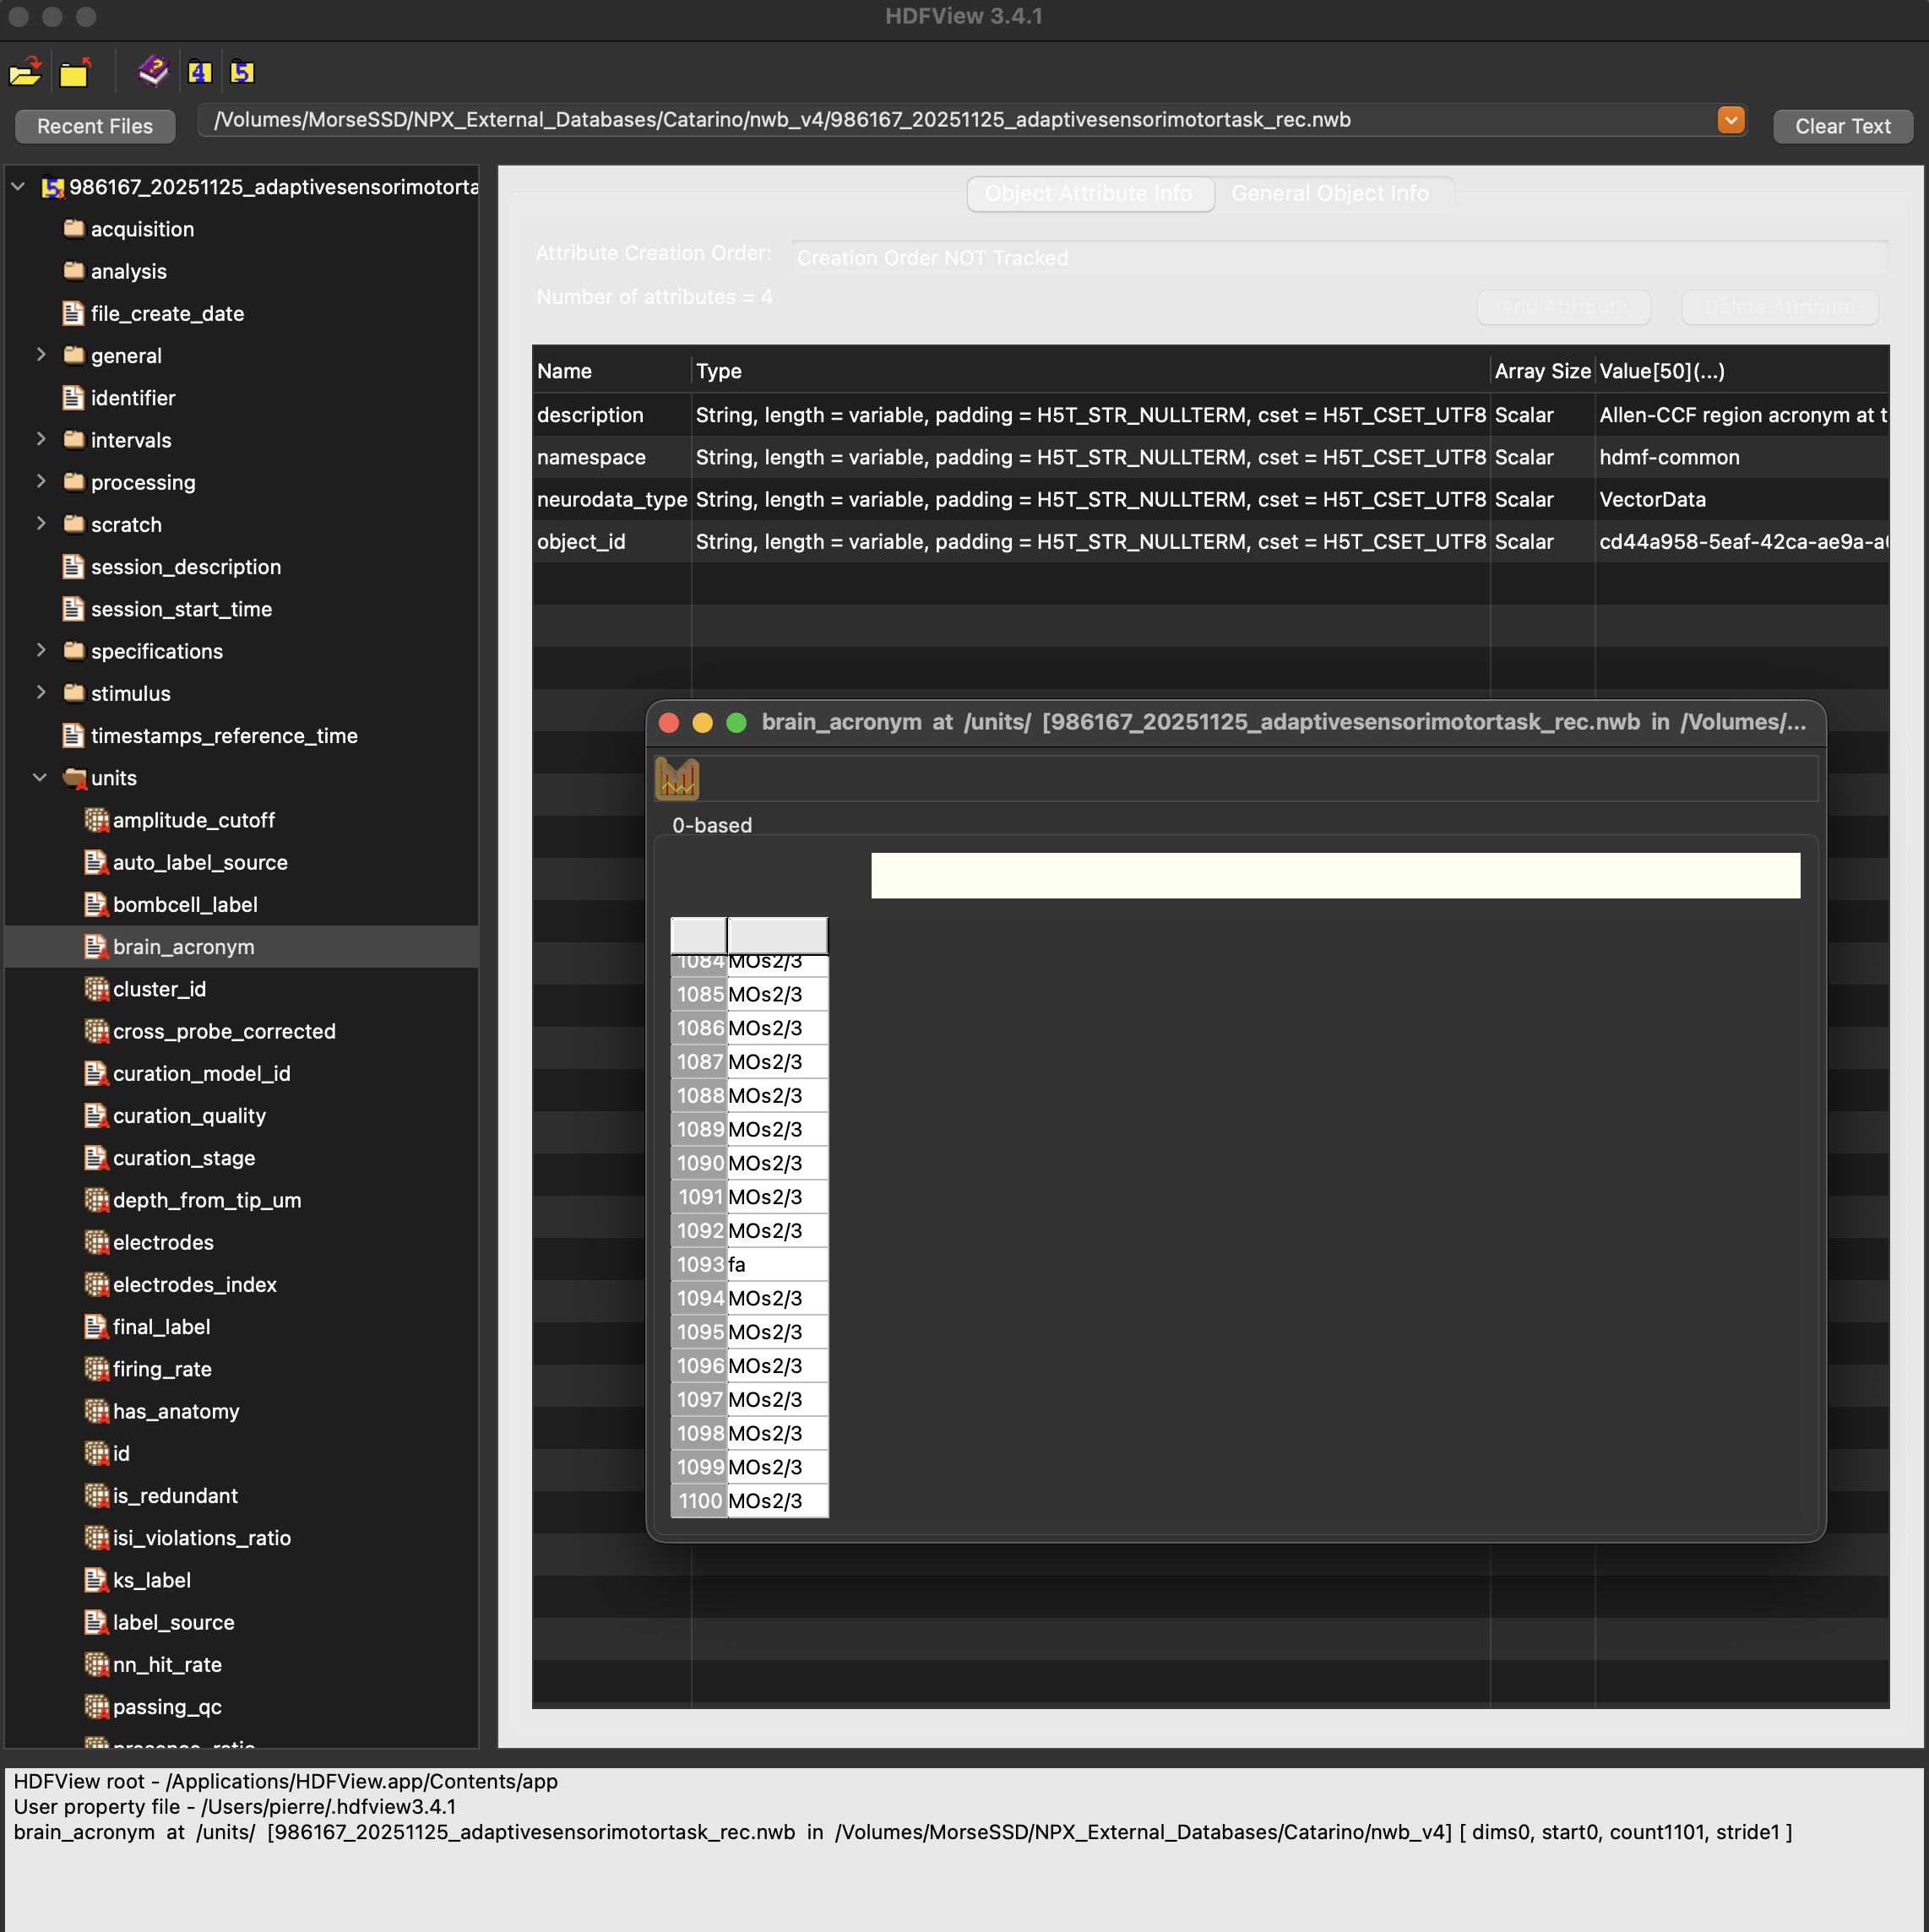
\includegraphics[width=6cm]{figures/hdfview.png}
			\end{center}
\end{frame} 

\begin{frame}
\frametitle{Explore NWB data - Neurosift}
			\begin{center}
			\url{https://neurosift.app/}\\
				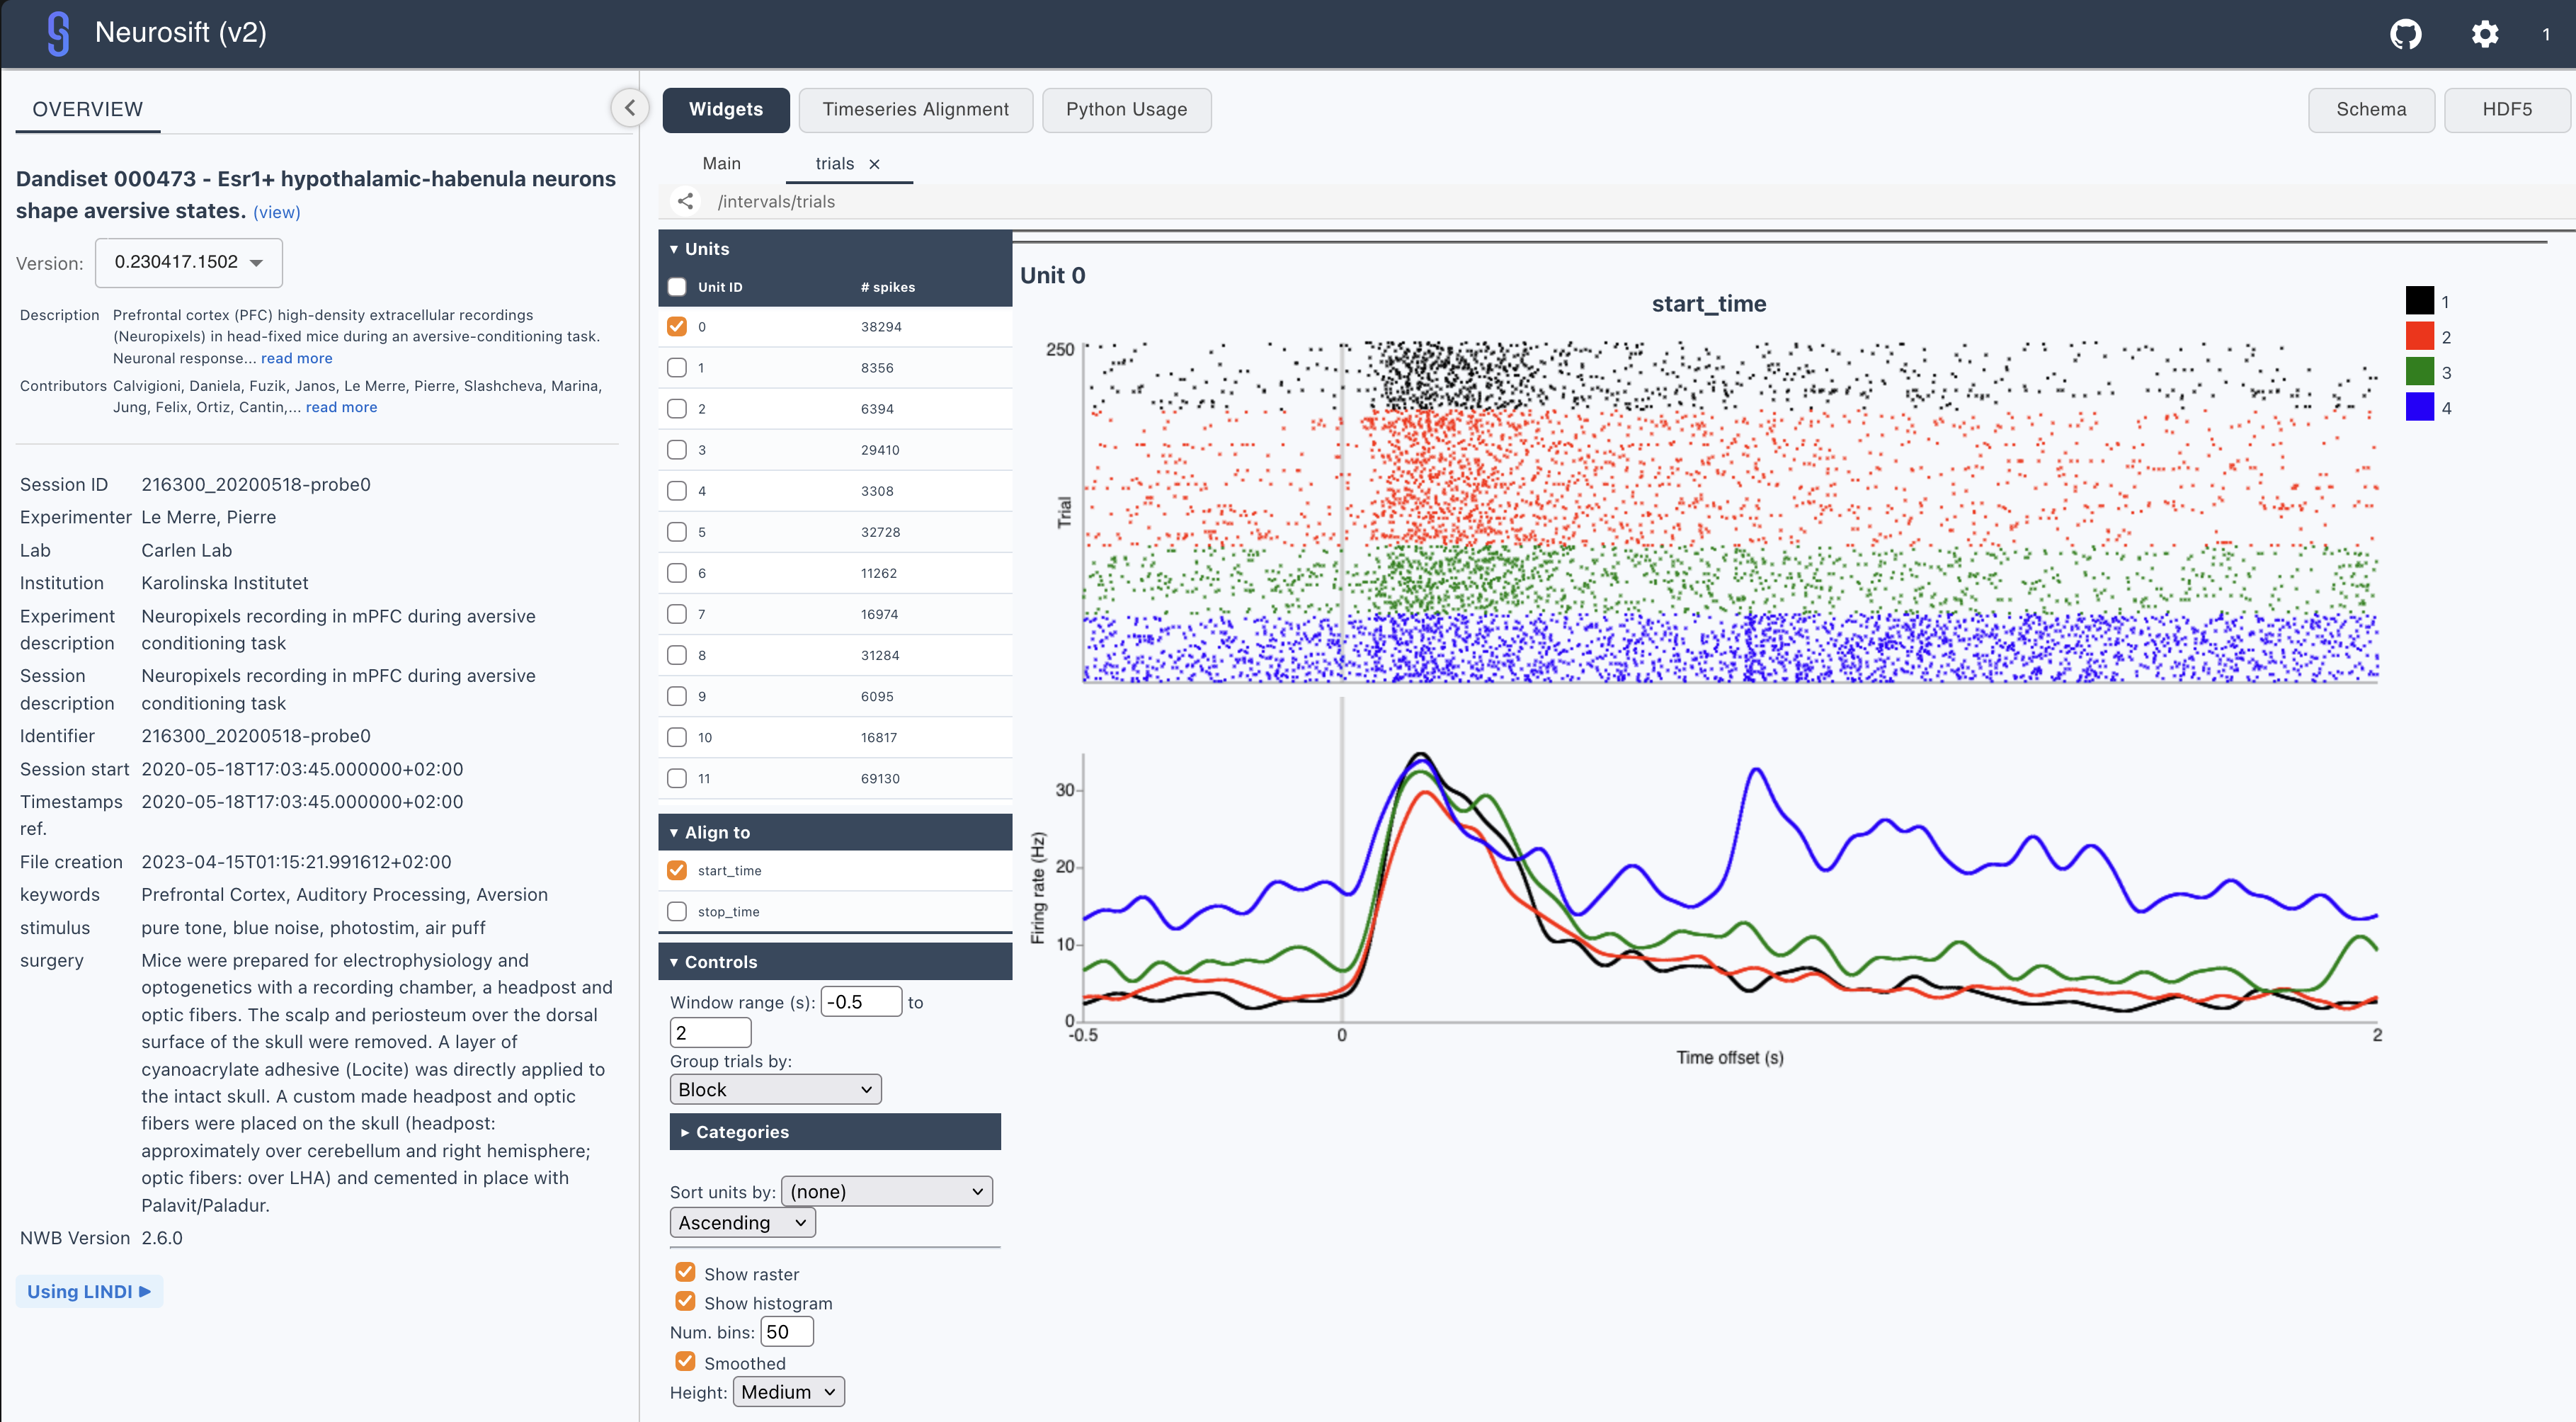
\includegraphics[width=10cm]{figures/neurosift.png}
			\end{center}
\end{frame} 

\begin{frame}
\frametitle{Explore NWB data - where are my spike times?}
			\begin{center}
				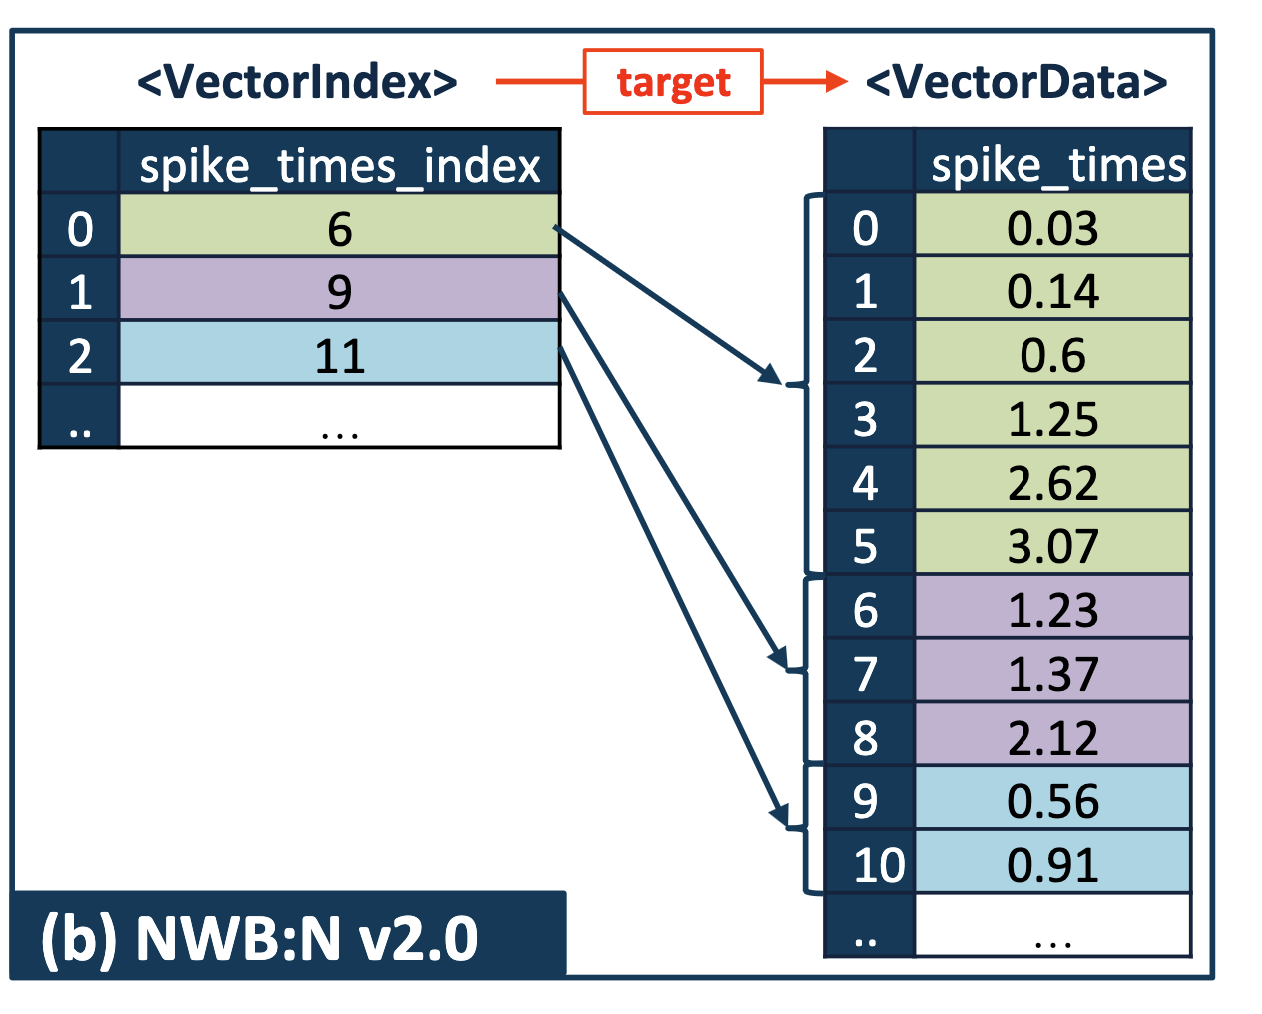
\includegraphics[width=8cm]{figures/ragged.png}
			\end{center}
\end{frame} 


 %%%%%%%%%%%%%%%%%%%%%%%%%%%%%%%%%%%%%%%%%%%%%%%%%%%%%%%%%%%%%%%%%%%%%%%%%%%%%

\section[Rates and intervals]{Spike rates and intervals}


\begin{frame}
\frametitle{Spike trains are Point processes}
			\begin{center}
				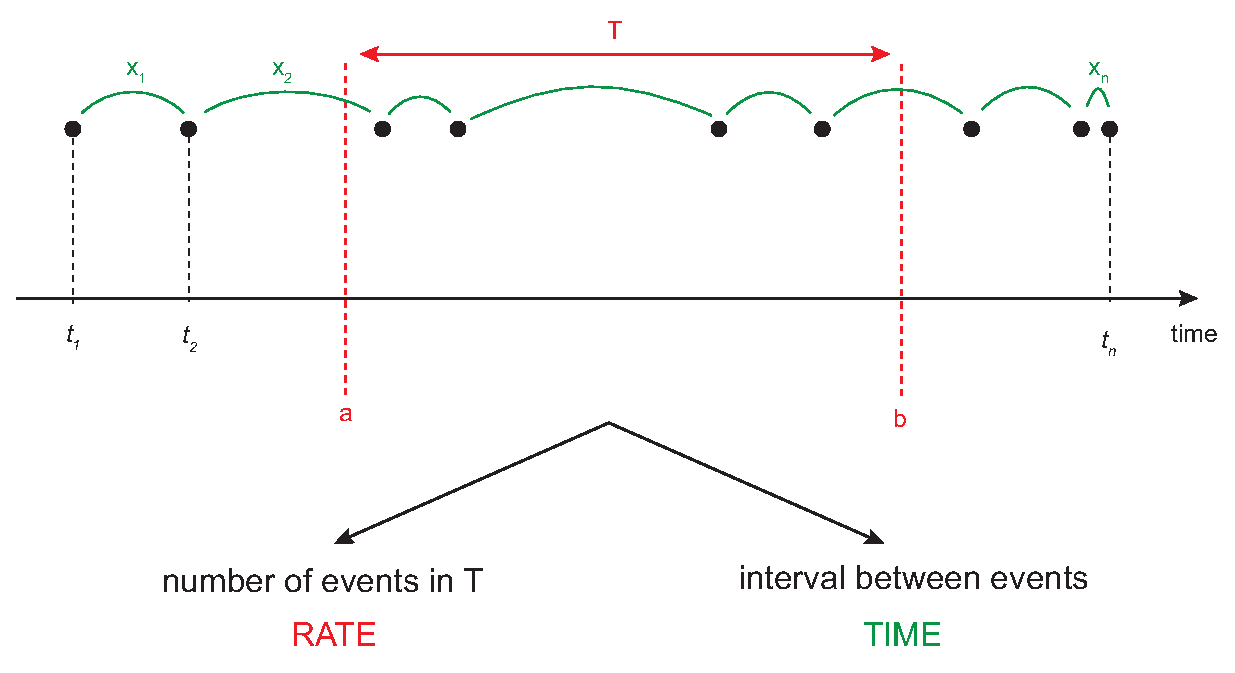
\includegraphics[width=10cm]{figures/timerate.eps}
			\end{center}
\end{frame} 




 %%%%%%%%%%%%%%%%%%%%%%%%%%%%%%%%%%%%%%%%%%%%%%%%%%%%%%%%%%%%%%%%%%%%%%%%%%%%%

\section[Waveforms and cell types]{Waveforms and cell types}

\begin{frame}
	\frametitle{Title}
		\begin{center}
			%\includegraphics[width=12.5cm]{myfigure.eps}
	\end{center}
\end{frame} 

 %%%%%%%%%%%%%%%%%%%%%%%%%%%%%%%%%%%%%%%%%%%%%%%%%%%%%%%%%%%%%%%%%%%%%%%%%%%%%

\section[Connectivity and Cross correlograms]{Connectivity and Cross correlograms}

\begin{frame}
	\frametitle{Title}
		\begin{center}
			%\includegraphics[width=12.5cm]{myfigure.eps}
	\end{center}
\end{frame} 

 %%%%%%%%%%%%%%%%%%%%%%%%%%%%%%%%%%%%%%%%%%%%%%%%%%%%%%%%%%%%%%%%%%%%%%%%%%%%%

\section[Population coding and embedding]{Population coding and embedding}

\begin{frame}
	\frametitle{Title}
		\begin{center}
			%\includegraphics[width=12.5cm]{myfigure.eps}
	\end{center}
\end{frame} 

 %%%%%%%%%%%%%%%%%%%%%%%%%%%%%%%%%%%%%%%%%%%%%%%%%%%%%%%%%%%%%%%%%%%%%%%%%%%%%

\section[Decoding]{Decoding}

\begin{frame}
	\frametitle{Title}
		\begin{center}
			%\includegraphics[width=12.5cm]{myfigure.eps}
	\end{center}
\end{frame} 

 %%%%%%%%%%%%%%%%%%%%%%%%%%%%%%%%%%%%%%%%%%%%%%%%%%%%%%%%%%%%%%%%%%%%%%%%%%%%%

\section[Conclusion]{Conclusion}


\begin{frame}
	\frametitle{Title}
		\begin{center}
			%\includegraphics[width=12.5cm]{myfigure.eps}
	\end{center}
\end{frame} 

\begin{frame}[plain]
\begin{columns}
\column{\dimexpr\paperwidth-10pt}
%\includegraphics[width=15.5cm]{my_big_image.png}
\end{columns}
\end{frame} 



\end{document}